%%%%%%%%%%%%%%%%%%%%%%%%%%%%%%%%%%%%%%%%%%%%%%%%%%%%%%%%%%%%%%%%%%%%%%%%

\begin{slide}{}
\normalsize

\begin{center}
3--Knoten 
\end{center}
\vspace*{0.5cm}

\footnotesize
\begin{enumerate}
\item 3--Knoten mit S\"ohnen der H\"ohe $h$ gibt Baum der H\"ohe $h+1$:

\hspace*{3cm} \epsfig{file=3-node.ps}
\begin{enumerate}
\item $k1 < k2$
\item alle Schl\"ussel im Teilbaum $l$ kleiner als $k1$
\item $k1$ kleiner als alle Schl\"ussel im Teilbaum $m$ 
\item alle Schl\"ussel im Teilbaum $m$ kleiner als $k2$
\item $k2$ kleiner als alle Schl\"ussel im Teilbaum $r$  
\item $l$ ist 2--3--4 Baum der H\"ohe $h$
\item $m$ ist 2--3--4 Baum der H\"ohe $h$
\item $r$ ist 2--3--4 Baum der H\"ohe $h$
\end{enumerate}

$$ l < k1 < m < k2 < r  $$
\end{enumerate}


\vspace*{\fill}
\tiny \addtocounter{mypage}{1}
\rule{17cm}{1mm}
2--3--4 B\"aume  \hspace*{\fill} Seite \arabic{mypage}
\end{slide}

%%%%%%%%%%%%%%%%%%%%%%%%%%%%%%%%%%%%%%%%%%%%%%%%%%%%%%%%%%%%%%%%%%%%%%%%

\begin{slide}{}
\normalsize

\begin{center}
4--Knoten 
\end{center}
\vspace*{0.5cm}

\footnotesize
\begin{enumerate}
\item[4.] 4--Knoten der H\"ohe $h+1$

\hspace*{1cm} \epsfig{file=4-node.ps}
\begin{enumerate}
\item $k1 < k2$
\item $k2 < k3$
\item alle Schl\"ussel im Teilbaum $l$ kleiner als $k1$
\item $k1$ kleiner als alle Schl\"ussel im Teilbaum $ml$ 
\item alle Schl\"ussel im Teilbaum $ml$ kleiner als $k2$
\item $k2$ kleiner als alle Schl\"ussel im Teilbaum $mr$  
\item alle Schl\"ussel im Teilbaum $mr$ kleiner als $k3$
\item $k3$ kleiner als alle Schl\"ussel im Teilbaum $r$  
\item $l$ \ \, ist 2--3--4 Baum der H\"ohe $h$
\item $ml$  ist 2--3--4 Baum der H\"ohe $h$
\item $mr$  ist 2--3--4 Baum der H\"ohe $h$
\item $r$ \ \, ist 2--3--4 Baum der H\"ohe $h$
\end{enumerate}

$$ l < k1 < ml < k2 < mr < k3 < r $$
\end{enumerate}

\vspace*{\fill}
\tiny \addtocounter{mypage}{1}
\rule{17cm}{1mm}
2--3--4 B\"aume  \hspace*{\fill} Seite \arabic{mypage}
\end{slide}

%%%%%%%%%%%%%%%%%%%%%%%%%%%%%%%%%%%%%%%%%%%%%%%%%%%%%%%%%%%%%%%%%%%%%%%%

\begin{slide}{}
\normalsize

\begin{center}
M\"ogliche Repr\"asentation der Knoten in \texttt{C}
\end{center}
\vspace*{0.5cm}

\footnotesize
\begin{verbatim}
typedef enum { TWO, THREE, FOUR } NodeType;
typedef struct Node* NodePtr;

struct Node {
    NodeType type;
    Key      key1;
    Value    val1;
    Key      key2;
    Value    val2;
    Key      key3;
    Value    val3;
    NodePtr  ptr1;
    NodePtr  ptr2;
    NodePtr  ptr3;
    NodePtr  ptr4;
    unsigned label;   // used only for printing
};
typedef NodePtr Tree;
\end{verbatim}
Interpretation von \texttt{type}:
\begin{enumerate}
\item \texttt{type == TWO}:   2--Knoten
\item \texttt{type == THREE}: 3--Knoten
\item \texttt{type == FOUR}:  4--Knoten
\end{enumerate}

\textbf{Vorteil} dieser Repr\"asentation: konzeptuell einfach

\textbf{Nachteil}: verbraucht zuviel Platz, denn 2--Knoten
verbraucht genauso viel Platz wie 4--Knoten.


\vspace*{\fill}
\tiny \addtocounter{mypage}{1}
\rule{17cm}{1mm}
2--3--4 B\"aume  \hspace*{\fill} Seite \arabic{mypage}
\end{slide}

%%%%%%%%%%%%%%%%%%%%%%%%%%%%%%%%%%%%%%%%%%%%%%%%%%%%%%%%%%%%%%%%%%%%%%%%

\begin{slide}{}
\normalsize

\begin{center}
Suche in 2--3--4--B\"aumen
\end{center}
\vspace*{0.5cm}

\footnotesize
Suche konzeptuell wie in bin\"aren B\"aumen, aber mehr F\"alle:
\begin{enumerate}
\item 2--Knoten mit Schl\"ussel $k$

      \hspace*{3cm} \epsfig{file=2a-node.ps}
      \vspace*{-0.7cm}

      \begin{enumerate}
      \item $k < k1$: Suche in $l$
      \item $k = k1$: Fertig, Wert gefunden!
      \item $k > k1$: Suche in $r$
      \end{enumerate}
\item 3--Knoten mit Schl\"ussel $k1$ und $k2$

      \hspace*{3cm} \epsfig{file=3-node.ps}
      \vspace*{-0.7cm}

      \begin{enumerate}
      \item $k < k1$: Suche in $l$
      \item $k = k1$: Fertig, Wert gefunden!
      \item $k > k1 \wedge k < k2$: Suche in $m$
      \item $k = k2$: Fertig, Wert gefunden!
      \item $k > k2$: Suche in $r$
      \end{enumerate}
\end{enumerate}

\vspace*{\fill}
\tiny \addtocounter{mypage}{1}
\rule{17cm}{1mm}
2--3--4 B\"aume  \hspace*{\fill} Seite \arabic{mypage}
\end{slide}

%%%%%%%%%%%%%%%%%%%%%%%%%%%%%%%%%%%%%%%%%%%%%%%%%%%%%%%%%%%%%%%%%%%%%%%%

\begin{slide}{}
\normalsize

\begin{center}
Suche in 2--3--4--B\"aumen (Fortsetzung)
\end{center}
\vspace*{0.5cm}

\footnotesize
\begin{enumerate}
\item[4.] 4--Knoten mit Schl\"ussel $k1$ und $k2$

      \hspace*{2cm} \epsfig{file=4-node.ps}

      \begin{enumerate}
      \item $k < k1$: Suche in $l$
      \item $k = k1$: Fertig, Wert gefunden!
      \item $k > k1 \wedge k < k2$: Suche in $ml$
      \item $k = k2$: Fertig, Wert gefunden!
      \item $k > k2 \wedge k < k3$: Suche in $mr$
      \item $k = k3$: Fertig, Wert gefunden!
      \item $k > k3$: Suche in $r$
      \end{enumerate}
\end{enumerate}

Bei Suche sind pro Knoten bis zu 3 Vergleiche notwendig.

\textbf{Aufwand} der Suche: $\Oh(h)$, falls $h$ H\"ohe des 2--3--4 Baums

Ein 2--3--4--Baum der H\"ohe $h$ hat mindestens $n = 2^h - 1$ Knoten!

Also gilt $h = \log_2(n+1)$, und damit haben wir:

\begin{center}
\framebox{\framebox{Suche in 2--3--4--Baum immer logarithmisch!}}  
\end{center}

\vspace*{\fill}
\tiny \addtocounter{mypage}{1}
\rule{17cm}{1mm}
2--3--4 B\"aume  \hspace*{\fill} Seite \arabic{mypage}
\end{slide}

%%%%%%%%%%%%%%%%%%%%%%%%%%%%%%%%%%%%%%%%%%%%%%%%%%%%%%%%%%%%%%%%%%%%%%%%

\begin{slide}{}
\normalsize

\begin{center}
    Suche in 2--3--4--B\"aumen (Implementierung)
\end{center}
\vspace*{0.5cm}

\footnotesize
\begin{verbatim}
// Search for a given key in the ordered 2-3-4 tree t.
Value* search(Table t, Key key) 
{
    if (t == 0) return 0;
    switch (t->type) {
    case TWO: {
        int cmp = compareKey(key, t->key1);
        if (cmp == -1) {
            return search(t->ptr1, key);
        } else if (cmp == 0) {
            return &(t->val1);
        } 
        assert(cmp == 1);
        return search(t->ptr2, key);
    }
    case THREE: {
        int cmp1 = compareKey(key, t->key1);
        if (cmp1 == -1) {
            return search(t->ptr1, key);
        } else if (cmp1 == 0) {
            return &(t->val1);
        } 
        assert(cmp1 == 1);
        int cmp2 = compareKey(key, t->key2);
        if (cmp2 == -1) {
            return search(t->ptr2, key);
        } else if (cmp2 == 0) {
            return &(t->val2);
        }
        assert(cmp2 == 1);
        return search(t->ptr3, key);
    }
    ...
\end{verbatim}


\vspace*{\fill}
\tiny \addtocounter{mypage}{1}
\rule{17cm}{1mm}
2--3--4 B\"aume  \hspace*{\fill} Seite \arabic{mypage}
\end{slide}

%%%%%%%%%%%%%%%%%%%%%%%%%%%%%%%%%%%%%%%%%%%%%%%%%%%%%%%%%%%%%%%%%%%%%%%%

\begin{slide}{}
\normalsize

\begin{center}
    Implementierung der Suche (Fortsetzung)
\end{center}
\vspace*{0.5cm}

\footnotesize
\begin{verbatim}
    case FOUR: {
        int cmp1 = compareKey(key, t->key1);
        if (cmp1 == -1) {
            return search(t->ptr1, key);
        } else if (cmp1 == 0) {
            return &(t->val1);
        } 
        assert(cmp1 == 1);
        int cmp2 = compareKey(key, t->key2);
        if (cmp2 == -1) {
            return search(t->ptr2, key);
        } else if (cmp2 == 0) {
            return &(t->val2);
        }
        assert(cmp2 == 1);
        int cmp3 = compareKey(key, t->key3);
        if (cmp3 == -1) {
            return search(t->ptr3, key);
        } else if (cmp3 == 0) {
            return &(t->val3);
        }
        assert(cmp3 == 1);
        return search(t->ptr4, key);
    }
    }
    //  added to avoid a compiler warning.
    assert(0);
    return 0;
}
\end{verbatim}

\vspace*{\fill}
\tiny \addtocounter{mypage}{1}
\rule{17cm}{1mm}
2--3--4 B\"aume  \hspace*{\fill} Seite \arabic{mypage}
\end{slide}

%%%%%%%%%%%%%%%%%%%%%%%%%%%%%%%%%%%%%%%%%%%%%%%%%%%%%%%%%%%%%%%%%%%%%%%%

\begin{slide}{}
\normalsize

\begin{center}
Einf\"ugen in 2--3--4 B\"aumen
\end{center}
\vspace*{0.5cm}

\footnotesize
Algorithmus zum Einf\"ugen von gegebenen $\langle \textsl{key}, \textsl{val} \rangle$ Paar
\begin{enumerate}
\item Suche nach Schl\"ussel \textsl{key} bis Blatt erreicht ist

      (Ein Blatt ist ein 2--3--4--Baum der H\"ohe 1)
\item Fall--Unterscheidung nach Art des Blattes:
      \begin{enumerate}
      \item Blatt ist 2--Knoten: f\"uge $\langle \textsl{key}, \textsl{val} \rangle$ ein

            Neues Blatt ist 3--Knoten

\epsfig{file=ex1.ps} \raisebox{2cm}{ \ 1 einf\"ugen \ }  \epsfig{file=ex2.ps}         
      \item Blatt ist 3--Knoten: f\"uge $\langle \textsl{key}, \textsl{val} \rangle$ ein

            Neues Blatt ist 4--Knoten 
            \vspace*{0.5cm}

            Beispiel: oben 7 einf\"ugen

            \hspace*{2cm} \epsfig{file=ex3.ps}
      \end{enumerate}
      \item Blatt ist 4--Knoten: Pech gehabt!
\end{enumerate}

\vspace*{\fill}
\tiny \addtocounter{mypage}{1}
\rule{17cm}{1mm}
2--3--4 B\"aume  \hspace*{\fill} Seite \arabic{mypage}
\end{slide}

%%%%%%%%%%%%%%%%%%%%%%%%%%%%%%%%%%%%%%%%%%%%%%%%%%%%%%%%%%%%%%%%%%%%%%%%

\begin{slide}{}
\normalsize

\begin{center}
Einf\"ugen in 2--3--4 B\"aume (Fortsetzung)
\end{center}
\vspace*{0.5cm}

\footnotesize
Einf\"ugen in 4--Knoten: Erster Versuch

\raisebox{2.6cm}{\epsfig{file=ex3.ps}} \raisebox{3.4cm}{ \ 5 einf\"ugen \ }  \epsfig{file=ex4.ps}

Geht nicht: Teilb\"aume haben unterschiedliche H\"ohe!
\vspace*{0.5cm}

\begin{center}
\framebox{\framebox{ 2--3--4 B\"aume k\"onnen nicht nach unten wachsen!}}  
\end{center}
\vspace*{0.5cm}

Zweiter Versuch: 4--Knoten aufspalten:

\hspace*{1.3cm} \raisebox{1.6cm}{
\epsfig{file=ex5.ps}} \raisebox{2.4cm}{ \ aufspalten \ }  \epsfig{file=ex6.ps}

Dann Schl\"ussel 6 nach oben schieben!

\vspace*{\fill}
\tiny \addtocounter{mypage}{1}
\rule{17cm}{1mm}
2--3--4 B\"aume  \hspace*{\fill} Seite \arabic{mypage}
\end{slide}

%%%%%%%%%%%%%%%%%%%%%%%%%%%%%%%%%%%%%%%%%%%%%%%%%%%%%%%%%%%%%%%%%%%%%%%%

\begin{slide}{}
\normalsize

\begin{center}
Einf\"ugen in 2--3--4 B\"aume (Fortsetzung)
\end{center}
\vspace*{0.5cm}

\footnotesize
Schl\"ussel 6 nach oben schieben: Ausgangspunkt

\hspace*{2.3cm} \epsfig{file=ex7.ps} 

Das ist kein 2--3--4 Baum, kann aber repariert werden, wenn
Knoten mit 6 nach oben geschoben werden kann!

\hspace*{2.3cm} \epsfig{file=ex8.ps} 

Jetzt einf\"ugen von 5 m\"oglich!

\hspace*{2.3cm} \epsfig{file=ex9.ps} 

\vspace*{\fill}
\tiny \addtocounter{mypage}{1}
\rule{17cm}{1mm}
2--3--4 B\"aume  \hspace*{\fill} Seite \arabic{mypage}
\end{slide}

%%%%%%%%%%%%%%%%%%%%%%%%%%%%%%%%%%%%%%%%%%%%%%%%%%%%%%%%%%%%%%%%%%%%%%%%

\begin{slide}{}
\normalsize

\begin{center}
Einf\"ugen in 2--3--4 B\"aume (Fortsetzung)
\end{center}
\vspace*{0.5cm}

\footnotesize
Neuer Algorithmus
\begin{enumerate}
\item Suche nach Schl\"ussel \textsl{key} bis Blatt erreicht ist

      Falls bei Suche 4--Knoten erreicht wird:
      \begin{enumerate}
      \item Spalte 4--Knoten auf
      \item Schiebe mittleren Schl\"ussel nach oben

            \textbf{Frage}: Warum geht das immer?
           
            (Problem wenn Knoten dar\"uber 4--Knoten ist)
            \vspace*{0.5cm}

            \textbf{Antwort}: Algorithmus stellt sicher, dass Knoten \"uber dem aktuellen
            Knoten nie 4--Knoten ist!
      \end{enumerate}
\item Falls Blatt erreicht ist, kann dies kein 4--Knoten sein:
      \begin{enumerate}
      \item Blatt ist 2--Knoten: f\"uge $\langle \textsl{key}, \textsl{val} \rangle$ ein

            Neues Blatt ist 3--Knoten

      \item Blatt ist 3--Knoten: f\"uge $\langle \textsl{key}, \textsl{val} \rangle$ ein

            Neues Blatt ist 4--Knoten 
      \end{enumerate}
\end{enumerate}

Baum w\"achst nur, wenn die Wurzel 4--Knoten ist und aufgespalten wird!


\vspace*{\fill}
\tiny \addtocounter{mypage}{1}
\rule{17cm}{1mm}
2--3--4 B\"aume  \hspace*{\fill} Seite \arabic{mypage}
\end{slide}

%%%%%%%%%%%%%%%%%%%%%%%%%%%%%%%%%%%%%%%%%%%%%%%%%%%%%%%%%%%%%%%%%%%%%%%%

\begin{slide}{}
\normalsize

\begin{center}
Wachstum  von 2--3--4 B\"aumen
\end{center}
\vspace*{0.5cm}

\footnotesize
\hspace*{2.3cm}  \epsfig{file=ex10.ps}

1. Schritt: aufspalten aller 4--Knoten bei Suche:

\hspace*{2.3cm} \epsfig{file=ex11.ps}

2. Schritt einf\"ugen von 2

\hspace*{2.3cm} \epsfig{file=ex12.ps}


\vspace*{\fill}
\tiny \addtocounter{mypage}{1}
\rule{17cm}{1mm}
2--3--4 B\"aume  \hspace*{\fill} Seite \arabic{mypage}
\end{slide}

%%%%%%%%%%%%%%%%%%%%%%%%%%%%%%%%%%%%%%%%%%%%%%%%%%%%%%%%%%%%%%%%%%%%%%%%

\begin{slide}{}
\normalsize

\begin{center}
Aufspaltens von 4--Knoten
\end{center}
\vspace*{0.5cm}

\footnotesize

Der 4--Knoten

\hspace*{1.3cm} \epsfig{file=4-node.ps}

wird durch Aufspalten zu

\hspace*{1.3cm} \epsfig{file=aufspalt.ps}


\vspace*{\fill}
\tiny \addtocounter{mypage}{1}
\rule{17cm}{1mm}
2--3--4 B\"aume  \hspace*{\fill} Seite \arabic{mypage}
\end{slide}

%%%%%%%%%%%%%%%%%%%%%%%%%%%%%%%%%%%%%%%%%%%%%%%%%%%%%%%%%%%%%%%%%%%%%%%%

\begin{slide}{}
\normalsize

\begin{center}
Implementierung des Aufspaltens
\end{center}
\vspace*{0.5cm}

\footnotesize
\begin{verbatim}
NodePtr split4Node(NodePtr t)
{
    assert(t->type == FOUR);
    // create the left node
    NodePtr left = malloc( sizeof(struct Node) );
    left->type = TWO;
    left->key1 = t->key1;
    left->val1 = t->val1;
    left->ptr1 = t->ptr1;
    left->ptr2 = t->ptr2;
    left->ptr3 = 0;
    left->ptr4 = 0;
    // create the right node
    NodePtr right = malloc( sizeof(struct Node) );
    right->type = TWO;
    right->key1 = t->key3;
    right->val1 = t->val3;
    right->ptr1 = t->ptr3;
    right->ptr2 = t->ptr4;
    right->ptr3 = 0;
    right->ptr4 = 0;
    // create the top node
    NodePtr top = malloc( sizeof(struct Node) );
    top->type = TWO;
    top->key1 = t->key2;
    top->val1 = t->val2;
    top->ptr1 = left;
    top->ptr2 = right;
    top->ptr3 = 0;
    top->ptr4 = 0;
    free(t);          // the old 4-node is disposed
    return top;
}
\end{verbatim}


\vspace*{\fill}
\tiny \addtocounter{mypage}{1}
\rule{17cm}{1mm}
2--3--4 B\"aume  \hspace*{\fill} Seite \arabic{mypage}
\end{slide}

%%%%%%%%%%%%%%%%%%%%%%%%%%%%%%%%%%%%%%%%%%%%%%%%%%%%%%%%%%%%%%%%%%%%%%%%

\begin{slide}{}
\normalsize

\begin{center}
Knoten nach oben schieben 
\end{center}
\vspace*{0.5cm}

\footnotesize
1. Fall: Vater--Knoten ist 2--Knoten, 4--Knoten ist links:

\hspace*{1.3cm} \epsfig{file=2-4-node-1.ps}

Aufspalten und Knoten nach oben schieben:

\hspace*{1.3cm} \epsfig{file=3-2-node-1.ps}


\vspace*{\fill}
\tiny \addtocounter{mypage}{1}
\rule{17cm}{1mm}
2--3--4 B\"aume  \hspace*{\fill} Seite \arabic{mypage}
\end{slide}

%%%%%%%%%%%%%%%%%%%%%%%%%%%%%%%%%%%%%%%%%%%%%%%%%%%%%%%%%%%%%%%%%%%%%%%%

\begin{slide}{}
\normalsize

\begin{center}
Knoten nach oben schieben 
\end{center}
\vspace*{0.5cm}

\footnotesize
2. Fall: Vater--Knoten ist 2--Knoten, 4--Knoten ist rechts:

\hspace*{1.3cm} \epsfig{file=2-4-node-2.ps}

Aufspalten und Knoten nach oben schieben:

\hspace*{1.3cm} \epsfig{file=3-2-node-2.ps}


\vspace*{\fill}
\tiny \addtocounter{mypage}{1}
\rule{17cm}{1mm}
2--3--4 B\"aume  \hspace*{\fill} Seite \arabic{mypage}
\end{slide}

%%%%%%%%%%%%%%%%%%%%%%%%%%%%%%%%%%%%%%%%%%%%%%%%%%%%%%%%%%%%%%%%%%%%%%%%

\begin{slide}{}
\normalsize

\begin{center}
Knoten nach oben schieben 
\end{center}
\vspace*{0.5cm}

\footnotesize
3. Fall: Vater--Knoten ist 3--Knoten, 4--Knoten ist 1. Sohn:

\hspace*{1.3cm} \epsfig{file=3-4-knoten-1.ps}

Aufspalten und Knoten nach oben schieben:

\hspace*{1.3cm} \epsfig{file=4-2-knoten-1.ps}


\vspace*{\fill}
\tiny \addtocounter{mypage}{1}
\rule{17cm}{1mm}
2--3--4 B\"aume  \hspace*{\fill} Seite \arabic{mypage}
\end{slide}

%%%%%%%%%%%%%%%%%%%%%%%%%%%%%%%%%%%%%%%%%%%%%%%%%%%%%%%%%%%%%%%%%%%%%%%%

\begin{slide}{}
\normalsize

\begin{center}
Knoten nach oben schieben 
\end{center}
\vspace*{0.5cm}

\footnotesize
4. Fall: Vater--Knoten ist 3--Knoten, 4--Knoten ist 2. Sohn:

\hspace*{1.3cm} \epsfig{file=3-4-knoten-2.ps}

Aufspalten und Knoten nach oben schieben:

\hspace*{1.3cm} \epsfig{file=4-2-knoten-2.ps}


\vspace*{\fill}
\tiny \addtocounter{mypage}{1}
\rule{17cm}{1mm}
2--3--4 B\"aume  \hspace*{\fill} Seite \arabic{mypage}
\end{slide}

%%%%%%%%%%%%%%%%%%%%%%%%%%%%%%%%%%%%%%%%%%%%%%%%%%%%%%%%%%%%%%%%%%%%%%%%

\begin{slide}{}
\normalsize

\begin{center}
Knoten nach oben schieben 
\end{center}
\vspace*{0.5cm}

\footnotesize
5. Fall: Vater--Knoten ist 3--Knoten, 4--Knoten ist 3. Sohn:

\hspace*{1.3cm} \epsfig{file=3-4-knoten-3.ps}

Aufspalten und Knoten nach oben schieben:

\hspace*{1.3cm} \epsfig{file=4-2-knoten-3.ps}


\vspace*{\fill}
\tiny \addtocounter{mypage}{1}
\rule{17cm}{1mm}
2--3--4 B\"aume  \hspace*{\fill} Seite \arabic{mypage}
\end{slide}

%%%%%%%%%%%%%%%%%%%%%%%%%%%%%%%%%%%%%%%%%%%%%%%%%%%%%%%%%%%%%%%%%%%%%%%%

\begin{slide}{}
\normalsize

\begin{center}
Knoten nach oben schieben (Implementierung)
\end{center}
\vspace*{0.5cm}

\footnotesize
Knoten ist 1. Sohn seines Vaters
\begin{verbatim}
void moveUp1(NodePtr t, NodePtr n) 
{
    assert(t != 0);
    assert(t->type != FOUR);
    assert(n->type == TWO);
    if (t->type == TWO) {
        t->key2 = t->key1;
        t->val2 = t->val1;
        t->key1 = n->key1;
        t->val1 = n->val1;
        t->ptr3 = t->ptr2;
        t->ptr1 = n->ptr1;
        t->ptr2 = n->ptr2;
        t->type = THREE;
        free(n);
        return;
    } 
    assert(t->type == THREE);
    t->key3 = t->key2;
    t->val3 = t->val2;
    t->key2 = t->key1;
    t->val2 = t->val1;
    t->key1 = n->key1;
    t->val1 = n->val1;
    t->ptr4 = t->ptr3;
    t->ptr3 = t->ptr2;
    t->ptr2 = n->ptr2;
    t->ptr1 = n->ptr1;
    t->type = FOUR;
    free(n);
    return;
}
\end{verbatim}

\vspace*{\fill}
\tiny \addtocounter{mypage}{1}
\rule{17cm}{1mm}
2--3--4 B\"aume  \hspace*{\fill} Seite \arabic{mypage}
\end{slide}

%%%%%%%%%%%%%%%%%%%%%%%%%%%%%%%%%%%%%%%%%%%%%%%%%%%%%%%%%%%%%%%%%%%%%%%%

\begin{slide}{}
\normalsize

\begin{center}
Knoten nach oben schieben (Implementierung)
\end{center}
\vspace*{0.5cm}

\footnotesize
Knoten ist 2. Sohn seines Vaters
\begin{verbatim}
void moveUp2(NodePtr t, NodePtr n) 
{
    assert(t != 0);
    assert(t->type != FOUR);
    assert(n->type == TWO);
    if (t->type == TWO) {
        t->key2 = n->key1;
        t->val2 = n->val1;
        t->ptr2 = n->ptr1;
        t->ptr3 = n->ptr2;
        t->type = THREE;
        free(n);
        return;
    } 
    assert(t->type == THREE);
    t->key3 = t->key2;
    t->val3 = t->val2;
    t->key2 = n->key1;
    t->val2 = n->val1;
    t->ptr4 = t->ptr3;
    t->ptr3 = n->ptr2;
    t->ptr2 = n->ptr1;
    t->type = FOUR;
    free(n);
    return;
}
\end{verbatim}

\vspace*{\fill}
\tiny \addtocounter{mypage}{1}
\rule{17cm}{1mm}
2--3--4 B\"aume  \hspace*{\fill} Seite \arabic{mypage}
\end{slide}

%%%%%%%%%%%%%%%%%%%%%%%%%%%%%%%%%%%%%%%%%%%%%%%%%%%%%%%%%%%%%%%%%%%%%%%%

\begin{slide}{}
\normalsize

\begin{center}
Knoten nach oben schieben (Implementierung)
\end{center}
\vspace*{0.5cm}

\footnotesize
Knoten ist 3. Sohn seines Vaters
\begin{verbatim}
void moveUp3(NodePtr t, NodePtr n) 
{
    assert(t != 0);
    assert(t->type == THREE);
    assert(n->type == TWO);
    t->key3 = n->key1;
    t->val3 = n->val1;
    t->ptr4 = n->ptr2;
    t->ptr3 = n->ptr1;
    t->type = FOUR;
    free(n);
    return;
}
\end{verbatim}

Auspalten von Knoten ist selten:
Wird ein Knoten eingef\"ugt, so muss im Mittel weniger als 1 Knoten 
aufgespaltet werden!

\vspace*{\fill}
\tiny \addtocounter{mypage}{1}
\rule{17cm}{1mm}
2--3--4 B\"aume  \hspace*{\fill} Seite \arabic{mypage}
\end{slide}

%%%%%%%%%%%%%%%%%%%%%%%%%%%%%%%%%%%%%%%%%%%%%%%%%%%%%%%%%%%%%%%%%%%%%%%%

\begin{slide}{}
\normalsize

\begin{center}
Einf\"ugen von Knoten (Implementierung)
\end{center}
\vspace*{0.5cm}

\footnotesize
Einf\"ugen im Blatt, betrachte zun\"achst 2--Knoten


\begin{verbatim}
void addKey(Tree p, Key key, Value val) {
    if (p->type == TWO) {
        int cmp = compareKey(key, p->key1);
        if (cmp == -1) {
            // move the old key to the right
            p->key2 = p->key1;
            p->val2 = p->val1;
            // insert the new key as first key
            p->key1 = key;
            p->val1 = val;
        } else {
            assert(cmp == 1);
            // insert the new key as second key
            p->key2 = key;
            p->val2 = val;
        }
        p->type = THREE;
        return;
    }
    ...
\end{verbatim}

\vspace*{\fill}
\tiny \addtocounter{mypage}{1}
\rule{17cm}{1mm}
2--3--4 B\"aume  \hspace*{\fill} Seite \arabic{mypage}
\end{slide}

%%%%%%%%%%%%%%%%%%%%%%%%%%%%%%%%%%%%%%%%%%%%%%%%%%%%%%%%%%%%%%%%%%%%%%%%

\begin{slide}{}
\normalsize

\begin{center}
Einf\"ugen im Blatt (3--Knoten)
\end{center}
\vspace*{0.5cm}

\footnotesize
\begin{verbatim}
    ...
    assert (p->type == THREE);
    int cmp1 = compareKey(key, p->key1);
    if (cmp1 == -1) {
        // move the old keys to the right
        p->key3 = p->key2;
        p->val3 = p->val2;
        p->key2 = p->key1;
        p->val2 = p->val1;
        // insert the new key as first key
        p->key1 = key;
        p->val1 = val;
    } else {
        assert(cmp1 == 1);
        int cmp2 = compareKey(key, p->key2);
        if (cmp2 == -1) {
            // move the second key right
            p->key3 = p->key2;
            p->val3 = p->val2;
            // insert the new key as second key
            p->key2 = key;
            p->val2 = val;
        } else {
            assert(cmp2 == 1);
            // insert the new key at the end
            p->key3 = key;
            p->val3 = val;
        }
    }
    p->type = FOUR;
    return;
}
\end{verbatim}


\vspace*{\fill}
\tiny \addtocounter{mypage}{1}
\rule{17cm}{1mm}
2--3--4 B\"aume  \hspace*{\fill} Seite \arabic{mypage}
\end{slide}

%%%%%%%%%%%%%%%%%%%%%%%%%%%%%%%%%%%%%%%%%%%%%%%%%%%%%%%%%%%%%%%%%%%%%%%%

\begin{slide}{}
\normalsize

\begin{center}
Einf\"ugen: Algorithmus
\end{center}
\vspace*{0.5cm}

\footnotesize
\textbf{Gegeben}: 
\begin{enumerate}
\item \texttt{t}:  Zeiger auf Wurzel--Knoten eines 2--3--4 Baums
\item \texttt{key}: Schl\"ussel, der eingef\"ugt werden soll
\item \texttt{val}: Wert, der mit Schl\"ussel assoziiert ist
\end{enumerate}
\textbf{Gesucht}: 2--3--4 Baum, der aus \texttt{*t} durch Einf\"ugen \\
\hspace*{2.8cm} von $\langle \mathtt{key}, \mathtt{val} \rangle$ hervorgeht.

\textbf{Algorithmus}:
\begin{enumerate}
\item Fall: Gegebener Baum ist leer
    
      Erzeuge neuen 2--Knoten mit Schl\"ussel \texttt{key}
\item Fall: Wurzel des gegebenen Baums ist 2--Knoten
  \begin{enumerate}
  \item Lokalisiere Teil--Baum, in den eingef\"ugt wird
  \item Falls Wurzel des Teil--Baums 4--Knoten: spalten
  \item F\"uge Schl\"ussel passend ein:
    \begin{itemize}
    \item Keine Aufspaltung: in Wurzel Teilbaum
    \item Aufspaltung: in gegebenem Baum \texttt{*t}
    \end{itemize}
  \end{enumerate}
\item Fall: Wurzel des gegebenen Baums ist 3--Knoten

      analog zum 2. Fall
\item Fall: Wurzel des gegebenen Baums ist 4--Knoten
  \begin{enumerate}
  \item Spalte Knoten auf
  \item F\"uge Schl\"ussel in neuer Wurzel ein
  \end{enumerate}
\end{enumerate}


\vspace*{\fill}
\tiny \addtocounter{mypage}{1}
\rule{17cm}{1mm}
2--3--4 B\"aume  \hspace*{\fill} Seite \arabic{mypage}
\end{slide}

%%%%%%%%%%%%%%%%%%%%%%%%%%%%%%%%%%%%%%%%%%%%%%%%%%%%%%%%%%%%%%%%%%%%%%%%

\begin{slide}{}
\normalsize

\begin{center}
Einf\"ugen: Implementierung
\end{center}
\vspace*{0.5cm}

\footnotesize
\begin{verbatim}
Table insert(Tree t, Key key, Value val) {
    // If the tree *t is empty, create a new node. 
    if (t == 0) {
        NodePtr node = malloc( sizeof(struct Node) );
        node->type = TWO;
        node->key1 = key;
        node->val1 = val;
        node->ptr1 = 0;
        node->ptr2 = 0;
        node->ptr3 = 0;
        node->ptr4 = 0;
        return node;
    }
    switch (t->type) {
    // find the appropriate subtree where the new key
    // needs to be inserted and split the root node
    // of this subtree if necessary
    case TWO: {
        int cmp = compareKey(key, t->key1);
        if (cmp == -1) {
            t = splitAndInsert(t, t->ptr1, key, val);
        } else if (cmp == 0) {
            t->val1 = val;
        } else {
            assert(cmp == 1);
            t = splitAndInsert(t, t->ptr2, key, val);
        }
        return t;
    }
    ...
\end{verbatim}


\vspace*{\fill}
\tiny \addtocounter{mypage}{1}
\rule{17cm}{1mm}
2--3--4 B\"aume  \hspace*{\fill} Seite \arabic{mypage}
\end{slide}

%%%%%%%%%%%%%%%%%%%%%%%%%%%%%%%%%%%%%%%%%%%%%%%%%%%%%%%%%%%%%%%%%%%%%%%%

\begin{slide}{}
\normalsize

\begin{center}
Einf\"ugen: Implementierung
\end{center}
\vspace*{0.5cm}

\footnotesize
Einf\"ugen in 3--Knoten und 4--Knoten
\begin{verbatim}
    ...
    case THREE: {
        int cmp1 = compareKey(key, t->key1);
        if (cmp1 == -1) {
            t = splitAndInsert(t, t->ptr1, key, val);
        } else if (cmp1 == 0) {
            t->val1 = val;
        } else {
            assert(cmp1 == 1);
            int cmp2 = compareKey(key, t->key2);
            if (cmp2 == -1) {
                t = splitAndInsert(t, t->ptr2, key, val);
            } else if (cmp2 == 0) {
                t->val2 = val;
            } else {
                assert(cmp2 == 1);
                t = splitAndInsert(t, t->ptr3, key, val);
            }
        }
        return t;
    }
    case FOUR: {
        NodePtr n = split4Node(t);
        return insert(n, key, val);
    }
    }
    // avoid compiler warning about missing return
    assert(0);
    return 0;
}
\end{verbatim}


\vspace*{\fill}
\tiny \addtocounter{mypage}{1}
\rule{17cm}{1mm}
2--3--4 B\"aume  \hspace*{\fill} Seite \arabic{mypage}
\end{slide}

%%%%%%%%%%%%%%%%%%%%%%%%%%%%%%%%%%%%%%%%%%%%%%%%%%%%%%%%%%%%%%%%%%%%%%%%

\begin{slide}{}
\normalsize

\begin{center}
Aufspalten und Einf\"ugen: Algorithmus
\end{center}
\vspace*{0.5cm}

\footnotesize
\textbf{Gegeben}: 
\begin{enumerate}
\item \texttt{p}, \texttt{t}: Knoten in 2--3--4 Baum
\item \texttt{p} is Vater von \texttt{t}
\item \texttt{key}: Schl\"ussel, der in \texttt{*t} eingef\"ugt werden soll
\item \texttt{val}: zugeh\"origer Wert
\end{enumerate}
\textbf{Algorithmus}:
\begin{enumerate}
\item Fall: \texttt{*t} ist leerer Baum

      $\langle \mathtt{key}, \mathtt{val} \rangle$ wird Blatt \texttt{*p} eingef\"ugt
\item Fall: \texttt{*t} ist 4--Knoten
      \begin{enumerate}
      \item Spalte Knoten auf \\[0.3cm]
            \hspace*{1.3cm} \texttt{NodePtr n = split4Node(t)}
      \item F\"uge $\langle \mathtt{key}, \mathtt{val} \rangle$ in \texttt{n} ein: \\[0.3cm]
            \hspace*{1.3cm} \texttt{insert(n, key, val)}
      \item Schiebe Knoten $n$ nach oben zu Vater--Knoten \\[0.3cm]
            \hspace*{1.3cm} \texttt{moveUp}$i$\texttt{(p, n)} \quad mit $i \in \{1,2,3\}$
      \end{enumerate}
\item Fall: Sonst f\"uge $\langle \mathtt{key}, \mathtt{val} \rangle$ in \texttt{t} ein: \\[0.3cm]
      \hspace*{1.3cm} \texttt{insert(n, key, val)}
\end{enumerate}

\vspace*{\fill}
\tiny \addtocounter{mypage}{1}
\rule{17cm}{1mm}
2--3--4 B\"aume  \hspace*{\fill} Seite \arabic{mypage}
\end{slide}

%%%%%%%%%%%%%%%%%%%%%%%%%%%%%%%%%%%%%%%%%%%%%%%%%%%%%%%%%%%%%%%%%%%%%%%%

\begin{slide}{}
\normalsize

\begin{center}
Aufspalten und Einf\"ugen: Implementierung
\end{center}
\vspace*{0.5cm}

\footnotesize
\begin{verbatim}
Tree splitAndInsert(NodePtr p, NodePtr t, Key key, Value val)
{
    // If the parent is a leaf, the key is inserted in
    // the parent.
    if (t == 0) {
        addKey(p, key, val);
        return p;
    }
    // If the root of the subtree where key is to be 
    // inserted is a 4-node, split the 4-node first, 
    // insert the key into the resulting tree, and 
    // finally move the middle key of the resulting 
    // tree into the parent node p.
    if (t->type == FOUR) {
        NodePtr n = split4Node(t);
        insert(n, key, val);
        if (t == p->ptr1) {
            moveUp1(p, n);
        } else if (t == p->ptr2) {
            moveUp2(p, n);
        } else {
            assert(t == p->ptr3);
            moveUp3(p, n);
        }
        return p;
    }
    insert(t, key, val);
    return p;
}
\end{verbatim}

\vspace*{\fill}
\tiny \addtocounter{mypage}{1}
\rule{17cm}{1mm}
2--3--4 B\"aume  \hspace*{\fill} Seite \arabic{mypage}
\end{slide}

%%%%%%%%%%%%%%%%%%%%%%%%%%%%%%%%%%%%%%%%%%%%%%%%%%%%%%%%%%%%%%%%%%%%%%%%

\begin{slide}{}
\normalsize

\begin{center}
Darstellung der Knoten als Union
\end{center}
\vspace*{0.5cm}

\footnotesize
\begin{verbatim}
typedef enum { TWO, THREE, FOUR } NodeType;
typedef struct Node* NodePtr;

typedef struct TwoNode*   TwoNodePtr;
typedef struct ThreeNode* ThreeNodePtr;
typedef struct FourNode*  FourNodePtr;

struct TwoNode {
    Key      key;
    Value    val;
    NodePtr  left;
    NodePtr  right;
    unsigned label;  // used for visualization
};

struct ThreeNode {
    Key      key1;
    Value    val1;
    Key      key2;
    Value    val2;
    NodePtr  left;
    NodePtr  middle;
    NodePtr  right;
    unsigned label;  // used for visualization
};
\end{verbatim}

\vspace*{\fill}
\tiny \addtocounter{mypage}{1}
\rule{17cm}{1mm}
2--3--4 B\"aume  \hspace*{\fill} Seite \arabic{mypage}
\end{slide}

%%%%%%%%%%%%%%%%%%%%%%%%%%%%%%%%%%%%%%%%%%%%%%%%%%%%%%%%%%%%%%%%%%%%%%%%

\begin{slide}{}
\normalsize

\begin{center}
Darstellung der Knoten als Union (Fortsetzung)
\end{center}
\vspace*{0.5cm}

\footnotesize
\begin{verbatim}
struct FourNode {
    Key      key1;
    Value    val1;
    Key      key2;
    Value    val2;
    Key      key3;
    Value    val3;
    NodePtr  left;
    NodePtr  middleLeft;
    NodePtr  middleRight;
    NodePtr  right;
    unsigned label;  // used for visualization
};

struct Node {
    NodeType type;
    union {
        TwoNodePtr   twoNodePtr;
        ThreeNodePtr threeNodePtr;
        FourNodePtr  fourNodePtr;
    } node;
};

typedef NodePtr Tree;
typedef Tree    Table;
\end{verbatim}

\vspace*{\fill}
\tiny \addtocounter{mypage}{1}
\rule{17cm}{1mm}
2--3--4 B\"aume  \hspace*{\fill} Seite \arabic{mypage}
\end{slide}

%%%%%%%%%%%%%%%%%%%%%%%%%%%%%%%%%%%%%%%%%%%%%%%%%%%%%%%%%%%%%%%%%%%%%%%%

\begin{slide}{}
\normalsize

\begin{center}
L\"oschen in 2--3--4 B\"aumen
\end{center}
\vspace*{0.5cm}

\footnotesize
Algorithmus zum L\"oschen von gegebenen Schl\"ussel $k$

Betrachte zun\"achst nur den Fall, dass $k$ in Blatt vorkommt
\begin{enumerate}
\item Suche nach Schl\"ussel $k$ bis Blatt erreicht ist

\item Fall--Unterscheidung nach Art des Blattes:
      \begin{enumerate}
      \item Blatt ist 4--Knoten: 
    
            
            Entferne Schl\"ussel, neues Blatt 3--Knoten

            \epsfig{file=ex3.ps} \raisebox{2.4cm}{l\"osche 7} \epsfig{file=ex2.ps}
    

      \item Blatt ist 3--Knoten: 

            Entferne Schl\"ussel, neues Blatt 2--Knoten

            \epsfig{file=ex2.ps} \raisebox{2.4cm}{l\"osche 1} \epsfig{file=ex1.ps}


      \end{enumerate}
      \item Blatt ist 2--Knoten: Pech gehabt!
\end{enumerate}

\vspace*{\fill}
\tiny \addtocounter{mypage}{1}
\rule{17cm}{1mm}
2--3--4 B\"aume  \hspace*{\fill} Seite \arabic{mypage}
\end{slide}

%%%%%%%%%%%%%%%%%%%%%%%%%%%%%%%%%%%%%%%%%%%%%%%%%%%%%%%%%%%%%%%%%%%%%%%%

\begin{slide}{}
\normalsize

\begin{center}
Behandlung von 2--Knoten beim L\"oschen
\end{center}
\vspace*{0.5cm}

\footnotesize
\begin{enumerate}
\item Beim Einf\"ugen waren 4--Knoten das Problem
\item L\"osung beim Einf\"ugen: 
  \begin{enumerate}
  \item Alle 4--Knoten auf dem Suchpfad  werden aufgespalten.
  \item Der dabei entstehende neue Knoten wird im Baum nach oben geschoben 
        und mit seinem Vater verschmolzen.
  \end{enumerate}
\item L\"osen beim L\"oschen analog:
  \begin{enumerate}
  \item Alle 2--Knoten auf dem Suchpfad werden in \\
        3--Knoten oder 4--Knoten transformiert.
  \item Wenn dann Blatt erreicht wird, kann dies kein \\
        2--Knoten sein.
  \end{enumerate}
\end{enumerate}
Um 2--Knoten in 3--Knoten oder 4--Knoten zu transformieren, gibt
es prinzipiell zwei M\"oglichkeiten:
\begin{enumerate}
\item Stehlen eines Schl\"ussels von unmittelbar benachbartem
      Schwester--Knoten
\item Fusionieren mit unmittelbar benachbartem Schwester--Knoten  
\end{enumerate}

\vspace*{\fill}
\tiny \addtocounter{mypage}{1}
\rule{17cm}{1mm}
2--3--4 B\"aume  \hspace*{\fill} Seite \arabic{mypage}
\end{slide}

%%%%%%%%%%%%%%%%%%%%%%%%%%%%%%%%%%%%%%%%%%%%%%%%%%%%%%%%%%%%%%%%%%%%%%%%


\begin{slide}{}
\normalsize

\begin{center}
Stehlen eines Schl\"ussels
\end{center}
\vspace*{0.5cm}

\footnotesize

 Knoten mit Sch\"ussel $k$  in 3--Knoten transformieren:

\hspace*{1.3cm} 
\epsfig{file=stehlen-2-node-1-von-2-vorher.ps}

Stehlen von $l1$ aus Nachbar--Knoten (Rotation)

\hspace*{1.3cm} 
\epsfig{file=stehlen-2-node-1-von-2-nachher.ps}



\vspace*{\fill}
\tiny \addtocounter{mypage}{1}
\rule{17cm}{1mm}
2--3--4 B\"aume  \hspace*{\fill} Seite \arabic{mypage}
\end{slide}

%%%%%%%%%%%%%%%%%%%%%%%%%%%%%%%%%%%%%%%%%%%%%%%%%%%%%%%%%%%%%%%%%%%%%%%%

\begin{slide}{}
\normalsize

\begin{center}
Stehlen eines Schl\"ussels (von links)
\end{center}
\vspace*{0.5cm}

\footnotesize

Knoten mit Sch\"ussel $k$  in 3--Knoten transformieren:

\hspace*{1.3cm} 
\epsfig{file=stehlen-2-node-2-von-1-vorher.ps}

Stehlen von $l1$ aus Nachbar--Knoten (Rotation)

\hspace*{1.3cm} 
\epsfig{file=stehlen-2-node-2-von-1-nachher.ps}



\vspace*{\fill}
\tiny \addtocounter{mypage}{1}
\rule{17cm}{1mm}
2--3--4 B\"aume  \hspace*{\fill} Seite \arabic{mypage}
\end{slide}

%%%%%%%%%%%%%%%%%%%%%%%%%%%%%%%%%%%%%%%%%%%%%%%%%%%%%%%%%%%%%%%%%%%%%%%%

\begin{slide}{}
\normalsize

\begin{center}
Stehlen eines Schl\"ussels (von 4--Knoten)
\end{center}
\vspace*{0.5cm}

\footnotesize

Knoten mit Sch\"ussel $k$  in 3--Knoten transformieren:

\hspace*{1.3cm} 
\epsfig{file=stehlen-2-node-1-von-2-4-node-vorher.ps}

Stehlen von $l1$ aus Nachbar--Knoten (Rotation)

\hspace*{1.3cm} 
\epsfig{file=stehlen-2-node-1-von-2-4-node-nachher.ps}



\vspace*{\fill}
\tiny \addtocounter{mypage}{1}
\rule{17cm}{1mm}
2--3--4 B\"aume  \hspace*{\fill} Seite \arabic{mypage}
\end{slide}

%%%%%%%%%%%%%%%%%%%%%%%%%%%%%%%%%%%%%%%%%%%%%%%%%%%%%%%%%%%%%%%%%%%%%%%%

\begin{slide}{}
\normalsize

\begin{center}
Stehlen eines Schl\"ussels
\end{center}
\vspace*{0.5cm}

\footnotesize
Beim Stehlen eines Schl\"ussels sind eine Reihe von Fallunterscheidungen
durchzuf\"uhren
\begin{enumerate}
\item Der Vater--Knoten ist ein 3--Knoten
      \begin{enumerate}
      \item Der unmittelbare Bruder ist erstes Kind
      \item Der unmittelbare Bruder ist zweites Kind
      \item Der unmittelbare Bruder ist drittes Kind
            \vspace*{0.5cm} 

      Jeder dieser F\"alle spaltet sich in 2 Unterf\"alle auf:
      \begin{itemize}
      \item Der unmittelbare Bruder ist 3--Knoten 
      \item Der unmittelbare Bruder ist 4--Knoten 
      \end{itemize}
      \end{enumerate}
\item Der Vater--Knoten ist ein 4--Knoten
      \begin{enumerate}
      \item Der unmittelbare Bruder ist erstes Kind
      \item Der unmittelbare Bruder ist zweites Kind
      \item Der unmittelbare Bruder ist drittes Kind
      \item Der unmittelbare Bruder ist viertes Kind
            \vspace*{0.5cm} 

       Auch hier haben wir dieselbe zus\"atzliche Aufspaltung wie oben
    \end{enumerate}
\end{enumerate}
Zus\"atzlich muss noch unterschieden werden, ob der Bruder rechts oder links
von dem Knoten liegt, der den Schl\"ussel stehlen will.

\begin{center}
\framebox{Insgesamt: 20 F\"alle!}  
\end{center}

\vspace*{\fill}
\tiny \addtocounter{mypage}{1}
\rule{17cm}{1mm}
2--3--4 B\"aume  \hspace*{\fill} Seite \arabic{mypage}
\end{slide}

%%%%%%%%%%%%%%%%%%%%%%%%%%%%%%%%%%%%%%%%%%%%%%%%%%%%%%%%%%%%%%%%%%%%%%%%

\begin{slide}{}
\normalsize

\begin{center}
Fusionieren
\end{center}
\vspace*{0.5cm}

\footnotesize
Knoten mit Sch\"ussel $k$  in 3--Knoten transformieren:

Stehlen nicht m\"oglich, weil unmittelbarer Bruder 2--Knoten

\hspace*{1.3cm} 
\epsfig{file=fusing-2-node-1-und-2-vorher.ps}

Knoten $k$ mit Bruder verschmelzen

\hspace*{1.3cm} 
\epsfig{file=fusing-2-node-1-und-2-nachher.ps}


\vspace*{\fill}
\tiny \addtocounter{mypage}{1}
\rule{17cm}{1mm}
2--3--4 B\"aume  \hspace*{\fill} Seite \arabic{mypage}
\end{slide}

%%%%%%%%%%%%%%%%%%%%%%%%%%%%%%%%%%%%%%%%%%%%%%%%%%%%%%%%%%%%%%%%%%%%%%%%

\begin{slide}{}
\normalsize

\begin{center}
Fusionieren (Vater ist 4--Knoten)
\end{center}
\vspace*{0.5cm}

\footnotesize
\footnotesize

\hspace*{1.3cm} 
\epsfig{file=fusing-4-node-1-und-2-vorher.ps}

Knoten $k$ mit Bruder verschmelzen

\hspace*{1.3cm} 
\epsfig{file=fusing-4-node-1-und-2-nachher.ps}

\vspace*{\fill}
\tiny \addtocounter{mypage}{1}
\rule{17cm}{1mm}
2--3--4 B\"aume  \hspace*{\fill} Seite \arabic{mypage}
\end{slide}

%%%%%%%%%%%%%%%%%%%%%%%%%%%%%%%%%%%%%%%%%%%%%%%%%%%%%%%%%%%%%%%%%%%%%%%%

\begin{slide}{}
\normalsize

\begin{center}
Fusionieren
\end{center}
\vspace*{0.5cm}

\footnotesize
Beim Fusionieren sind eine Reihe von Fallunterscheidungen
durchzuf\"uhren
\begin{enumerate}
\item Der Vater--Knoten ist ein 3--Knoten
      \begin{enumerate}
      \item Der unmittelbare Bruder ist erstes Kind
      \item Der unmittelbare Bruder ist zweites Kind
      \item Der unmittelbare Bruder ist drittes Kind
      \end{enumerate}
\item Der Vater--Knoten ist ein 4--Knoten
      \begin{enumerate}
      \item Der unmittelbare Bruder ist erstes Kind
      \item Der unmittelbare Bruder ist zweites Kind
      \item Der unmittelbare Bruder ist drittes Kind
      \item Der unmittelbare Bruder ist viertes Kind
    \end{enumerate}
\end{enumerate}
Zus\"atzlich muss noch unterschieden werden, ob der Bruder rechts oder links
von dem Knoten liegt, der den Schl\"ussel stehlen will.

\begin{center}
\framebox{Insgesamt: 10 F\"alle!}  
\end{center}


\vspace*{\fill}
\tiny \addtocounter{mypage}{1}
\rule{17cm}{1mm}
2--3--4 B\"aume  \hspace*{\fill} Seite \arabic{mypage}
\end{slide}

%%%%%%%%%%%%%%%%%%%%%%%%%%%%%%%%%%%%%%%%%%%%%%%%%%%%%%%%%%%%%%%%%%%%%%%%

\begin{slide}{}
\normalsize

\begin{center}
L\"oschen Allgemein
\end{center}
\vspace*{0.5cm}

\footnotesize
Bisher beschrieben: L\"oschen von Blatt--Knoten

Jetzt: L\"oschen von beliebigen Knoten
\begin{enumerate}
\item Ist Knoten $m$ Blatt?
\item Ja: l\"osche Knoten $m$, fertig
      \vspace*{0.4cm}

      Nein: 
\item Bestimme Nachfolger--Knoten $n$ von $m$

      Sei $k$ Schl\"ussel von $n$. Nachfolger--Knoten ist der Knoten $n$ mit Schl\"ussel $l$
      f\"ur den gilt:
      \begin{enumerate}
      \item $k < l$
      \item $l$ ist der kleinste Knoten im Baum mit $k < l$.
      \end{enumerate}
\item L\"osche $n$ (m\"oglich, da $o$ Blatt)
\item Schreibe $l$ und $v$ in Knoten $m$
\end{enumerate}
Komplexit\"at:  Ist $t$ eine 2--3--4--Baum mit $n$ Knoten, so betr\"agt der Aufwand f\"ur das
L\"oschen eines Knotens sowohl im schlechtesten als auch im besten Fall \\[0.6cm]
\hspace*{2.3cm} $\Oh\bigg(\log(n)\bigg)$


\vspace*{\fill}
\tiny \addtocounter{mypage}{1}
\rule{17cm}{1mm}
2--3--4 B\"aume  \hspace*{\fill} Seite \arabic{mypage}
\end{slide}

%%%%%%%%%%%%%%%%%%%%%%%%%%%%%%%%%%%%%%%%%%%%%%%%%%%%%%%%%%%%%%%%%%%%%%%%

\begin{slide}{}
\normalsize

\begin{center}
L\"oschen: Alternative Implementierung
\end{center}
\vspace*{0.5cm}

\footnotesize

\begin{enumerate}
\item F\"uhre zus\"atzliches Felder vom Type \texttt{bool} in der Struktur ein, die Knoten
      beschreibt.
\begin{verbatim}
    struct Node {
        NodeType type;
        bool     alive1;   
        Key      key1;
        Value    val1;
        bool     alive2;   
        Key      key2;
        Value    val2;
        bool     alive3;   
        Key      key3;
        Value    val3;
        ...
    };
\end{verbatim}
\item \texttt{alive == true}:   Schl\"ussel ist g\"ultig.
\item \texttt{alive == false}:  Schl\"ussel wurde gel\"oscht.
\item Verwalte au{\ss}erdem zwei globale Z\"ahler:
  \begin{enumerate}
  \item Anzahl aller g\"ultigen   Schl\"ussel
  \item Anzahl aller gel\"oschten Schl\"ussel
  \end{enumerate}
\item Falls mehr gel\"oschte  Schl\"ussel als g\"ultige Schl\"ussel existieren,
      baue Baum neu auf.

      Komplexit\"at f\"ur Baum mit $n$ Knoten:
      \begin{enumerate}
      \item Im schlimmsten Fall:           \hspace*{3.1cm} $\Oh(n)$
      \item Im statistischen Durchschnitt: \hspace*{0.3cm} $\Oh\bigg(\log(n)\bigg)$
      \end{enumerate}
\end{enumerate}

\vspace*{\fill}
\tiny \addtocounter{mypage}{1}
\rule{17cm}{1mm}
2--3--4 B\"aume  \hspace*{\fill} Seite \arabic{mypage}
\end{slide}

%%%%%%%%%%%%%%%%%%%%%%%%%%%%%%%%%%%%%%%%%%%%%%%%%%%%%%%%%%%%%%%%%%%%%%%%

\begin{slide}{}
\normalsize

\begin{center}
L\"oschen Alternative (Fortsetzung)
\end{center}
\vspace*{0.5cm}

\footnotesize
\begin{enumerate}
\item Zahl gel\"oschter Schl\"ussel gr\"o{\ss}er Zahl g\"ultiger Schl\"ussel?
\item Nein: Schl\"ussel suchen und als gel\"oscht markieren
\item Ja:
  \begin{enumerate}
  \item Sammle alle  g\"ultigen Schl\"ussel (nebst zugeh\"orige Werte) 
        aus dem Baum in 2 Feldern auf.
  \item L\"osche alten Baum.
  \item Baue neuen 2--3--4 Baum aus diesen Feldern auf.
  \end{enumerate}
\end{enumerate}

Aufsammeln:
\begin{verbatim}
void collectKeys(Tree t, unsigned* idx, 
                 Key keyArray[], Value valArray[]) 
{
    if (t == 0)
        return;
    switch (t->type) {
    case TWO: {
        collectKeys(t->ptr1, idx, keyArray, valArray);
        if (t->alive1) {
            keyArray[*idx] = t->key1;
            valArray[*idx] = t->val1;
            *idx = *idx + 1;
        }
        collectKeys(t->ptr2, idx, keyArray, valArray);
        return;
    }
    ...
\end{verbatim}


\vspace*{\fill}
\tiny \addtocounter{mypage}{1}
\rule{17cm}{1mm}
2--3--4 B\"aume  \hspace*{\fill} Seite \arabic{mypage}
\end{slide}

%%%%%%%%%%%%%%%%%%%%%%%%%%%%%%%%%%%%%%%%%%%%%%%%%%%%%%%%%%%%%%%%%%%%%%%%

\begin{slide}{}
\normalsize

\begin{center}
Baum neu Aufbauen
\end{center}
\vspace*{0.5cm}

\footnotesize
\textbf{Gegeben}:
\begin{enumerate}
\item \texttt{keyArray}: \textbf{geordnetes} Feld von Schl\"usseln
\item \texttt{valArray}: Feld der zugeh\"origen Schl\"ussel
\item \texttt{length}: L\"ange der Felder
\end{enumerate}
\textbf{Gesucht}: 2--3--4 Baum mit den Schl\"usseln aus \texttt{keyArray} 

Algorithmus
\begin{enumerate}
\item \texttt{length == 1}: erzeuge 2--Knoten
\item \texttt{length == 2}: erzeuge 3--Knoten
\item \texttt{length \% 2 == 1, length > 2}:
  \begin{enumerate}
  \item Setze \texttt{m = length/2}
  \item Rekursiv: Bilde Baum $l$ aus \\[0.3cm]
        \hspace*{1.3cm} $\underbrace{\texttt{keyArray[0]}, \; \cdots, \;\texttt{keyArray[m-1]}}_\mathtt{\displaystyle m}$
  \item Rekursiv: Bilde Baum $r$ aus \\[0.3cm]
        \hspace*{1.3cm} $\underbrace{\texttt{keyArray[m+1]},\; \cdots, \;\texttt{keyArray[m + m]}}_\mathtt{\displaystyle m}$
  \item Erzeuge 2--Knoten $n$ aus \\[0.3cm]
        \hspace*{1.3cm} $l$, $r$, $\texttt{keyArray[m]}$, $\mathtt{valArray[m]}$
  \item Gebe $n$ zur\"uck
  \end{enumerate}
\end{enumerate}

\vspace*{\fill}
\tiny \addtocounter{mypage}{1}
\rule{17cm}{1mm}
2--3--4 B\"aume  \hspace*{\fill} Seite \arabic{mypage}
\end{slide}

%%%%%%%%%%%%%%%%%%%%%%%%%%%%%%%%%%%%%%%%%%%%%%%%%%%%%%%%%%%%%%%%%%%%%%%%

\begin{slide}{}
\normalsize

\begin{center}
Baum neu Aufbauen (Fortsetzung)
\end{center}
\vspace*{0.5cm}

\footnotesize
\begin{enumerate}
\item[4.] \texttt{length \% 2 == 0, length > 2}:
  \begin{enumerate}
  \item Setze \texttt{m = length / 2 - 1}, also gilt \\[0.3cm]
        \hspace*{1.3cm} \texttt{length = m + 1 + 1 + m }
  \item Rekursiv: Bilde Baum $l$ aus \\[0.3cm]
        \hspace*{1.3cm} $\underbrace{\texttt{keyArray[0]}, \cdots, \texttt{keyArray[m-1]}}_\mathtt{\displaystyle m}$
  \item Rekursiv: Bilde Baum $r$ aus \\[0.3cm]
        \hspace*{1.3cm} $\underbrace{\texttt{keyArray[m+2]}, \cdots, \texttt{keyArray[m + m + 1]}}_\mathtt{\displaystyle m}$
  \item Erzeuge 2--Knoten $n$ aus \\[0.3cm]
        \hspace*{1.3cm} $l$, $r$, $\texttt{keyArray}[m]$, $\mathtt{valArray}[m]$
  \item F\"uge $\texttt{keyArray}[m+1]$, $\mathtt{valArray}[m+1]$ in $r$ ein \\[0.3cm]
        \hspace*{1.3cm} \texttt{res = insert(n, keyArray[m+1], valArray[m+1])}
  \item Gebe \texttt{res} zur\"uck
  \end{enumerate}
\end{enumerate}
\textbf{Wichtig}: Bei den beiden rekursiven Aufrufen muss die Zahl \\
\hspace*{2.7cm} der \"ubergebenen Schl\"ussel dieselbe sein!


\vspace*{\fill}
\tiny \addtocounter{mypage}{1}
\rule{17cm}{1mm}
2--3--4 B\"aume  \hspace*{\fill} Seite \arabic{mypage}
\end{slide}

%%%%%%%%%%%%%%%%%%%%%%%%%%%%%%%%%%%%%%%%%%%%%%%%%%%%%%%%%%%%%%%%%%%%%%%%

\begin{slide}{}
\normalsize

\begin{center}
\texttt{gdb} Command Line Interface
\end{center}
\vspace*{0.5cm}

\footnotesize
Aufruf
\begin{enumerate}
\item \texttt{gcc -std=c99 -Wall -lm {\bf -g} -o test-2-3-4 test-2-3-4.c}

      Ohne {\bf -g} wird beim Kompilieren keine Debug--Information erzeugt!
\item \texttt{gdb test-2-3-4}
\end{enumerate}

\texttt{gdb}--Kommandos
\begin{enumerate}
\item \texttt{break} \textsl{fctName}

       Anhalten bei Funktion \textsl{fctName}
\item \texttt{break} \textsl{lineNumber}

       Anhalten in Zeile \textsl{lineNumber}
\item \texttt{info breakpoints}

       zeigt Halte--Punkte und Beobachtungs--Punkte an
\item \texttt{delete} \textsl{number}

       l\"oscht  Halte--Punkt / Beobachtungs--Punkt

\item \texttt{display} \textsl{expr}

       wertet \underline{jedesmal} \textsl{expr} aus, druckt Ergebnis

       Beispiel: \texttt{display printTableDot(t, 42);}
\item \texttt{help}: 

       Liste der Topics, zu denen Hilfe existiert
\end{enumerate}

\vspace*{\fill}
\tiny \addtocounter{mypage}{1}
\rule{17cm}{1mm}
Debugging  \hspace*{\fill} Seite \arabic{mypage}
\end{slide}

%%%%%%%%%%%%%%%%%%%%%%%%%%%%%%%%%%%%%%%%%%%%%%%%%%%%%%%%%%%%%%%%%%%%%%%%

\begin{slide}{}
\normalsize

\begin{center}
\texttt{gdb} Kommandos
\end{center}
\vspace*{0.5cm}

\footnotesize
\begin{enumerate}
\item \texttt{run}:  startet das Programm
\item \texttt{continue}: 

      rechnet bis zum n\"achsten Haltepunkt
\item \texttt{step}:
      f\"uhrt eine Programm--Zeile aus
\item \texttt{next}:
      wie oben, springt \"uber Prozedur--Aufruf
\item \texttt{until} \textsl{line}

      Programm l\"auft bis zur spezifizierten Zeile
\item \texttt{finish}: 
      Programm l\"auft bis Ende aktueller Funktion
\item \texttt{print} \textsl{expr}

       gibt Ausdruck aus
\item \texttt{print} \textsl{fnct(arg1,...,argn)}

          wertet Benutzer--Funktion aus
    
       Beispiel: \texttt{p printTableDot(t, 42);}

\item \texttt{display} \textsl{expr}

      zeigt jedesmal \texttt{expr} an

      Beispiel: \texttt{display i}

\item \texttt{info display} 

      listet Ausdr\"ucke, die automatisch angezeigt werden
\item \texttt{delete display}: l\"oschen
\end{enumerate}

\vspace*{\fill}
\tiny \addtocounter{mypage}{1}
\rule{17cm}{1mm}
Debugging  \hspace*{\fill} Seite \arabic{mypage}
\end{slide}

%%%%%%%%%%%%%%%%%%%%%%%%%%%%%%%%%%%%%%%%%%%%%%%%%%%%%%%%%%%%%%%%%%%%%%%%

\begin{slide}{}
\normalsize

\begin{center}
Benutzung von \texttt{gdb} unter \textsl{XEmacs}
\end{center}
\vspace*{0.5cm}

\footnotesize
\begin{enumerate}
\item Aufruf Compiler: \texttt{Meta-x compile}
\item Aufruf Debugger: \texttt{Meta-x gdb}
\item Aufruf Shell:    \texttt{Meta-x shell}
\end{enumerate}
\vspace*{0.5cm}

Tastatur--Belegung \\[0.3cm]

\hspace*{1.3cm} 
\framebox{
  \begin{tabular}{|l|l|}
\hline
   command             & key sequence            \\
\hline
   \texttt{step}  & \fbox{Meta-s}             \rule[-12pt]{0pt}{34pt} \\
\hline
   \texttt{next}  & \fbox{Ctrl-c Ctrl-n}      \rule[-12pt]{0pt}{34pt} \\
\hline
   \texttt{continue}  & \fbox{Ctrl-c Meta-n}  \rule[-12pt]{0pt}{34pt} \\
\hline
   \texttt{finish}  & \fbox{Ctrl-c Ctrl-f}    \rule[-12pt]{0pt}{34pt} \\
\hline
   \texttt{break} \textsl{line}  & \fbox{Ctrl-x space} \rule[-12pt]{0pt}{34pt} \\
\hline
   n\"achstes Kommando  & \fbox{Meta-p} \rule[-12pt]{0pt}{34pt} \\
\hline
   letztes Kommando     & \fbox{Meta-n} \rule[-12pt]{0pt}{34pt} \\
\hline
   \texttt{up}  & \fbox{Ctrl-c \texttt{<}} \rule[-12pt]{0pt}{34pt} \\
\hline
   \texttt{down}  & \fbox{Ctrl-c \texttt{>}} \rule[-12pt]{0pt}{34pt} \\
\hline
  \end{tabular}}

Befehle sind ebenfalls \"uber GUI ausf\"uhrbar

\vspace*{\fill}
\tiny \addtocounter{mypage}{1}
\rule{17cm}{1mm}
Debugging  \hspace*{\fill} Seite \arabic{mypage}
\end{slide}


%%% Local Variables: 
%%% mode: latex
%%% TeX-master: "2-3-4.tex"
%%% End: 
